\documentclass[t,aspectratio=169]{beamer} % 使用16:9宽高比
\usetheme{Madrid} % 选择Madrid主题
\usecolortheme{default} % 使用默认颜色主题

% 设置字体
\usepackage[UTF8]{ctex}
\usefonttheme{structurebold} % 加粗结构字体

% 数学包
\usepackage{amsmath, amssymb, bm}
\usepackage{url}
\usepackage{booktabs}

% 图形包
\usepackage{graphicx}

% 标题页信息
\title[10.2.卷积滤波器]{第10章：卷积网络}
\subtitle{第2节：卷积滤波器 (Convolutional Filters)}
\author{《深度学习基础》课程小组}
% \institute{上海立信会计金融学院}
\date{\today}

\begin{document}

% 标题页
\frame{\titlepage}

% 目录页
\begin{frame}
    \frametitle{目录}
    \tableofcontents
\end{frame}

% ============================================================
% 第一部分：动机与四大概念
% ============================================================
\section{动机与四大概念}

\begin{frame}
    \frametitle{1. 全连接网络的参数灾难}
    \begin{itemize}
        \item 图像数据\alert{高维}，标准全连接架构需要\alert{海量参数}。
        \item 例：$10^3 \times 10^3$ 彩色图像（3 通道）+ 1000 隐藏单元
        \begin{itemize}
            \item 第一层权重：$3 \times 10^9$
        \end{itemize}
        \item 还必须\alert{通过样本学习}不变性和等变性 $\Rightarrow$ 需要巨大数据集。
        \item \textbf{解决思路}：设计架构融入\alert{图像结构的归纳偏置}。
        \begin{itemize}
            \item 大幅降低数据集需求
            \item 改善关于图像空间对称性的泛化
        \end{itemize}
    \end{itemize}
\end{frame}

\begin{frame}
    \frametitle{1.1 四大核心概念}
    利用图像二维结构创建归纳偏置：
    \begin{enumerate}
        \item \alert{层级性} (hierarchy)：从低级特征到高级概念
        \item \alert{局部性} (locality)：单元只看小区域
        \item \alert{等变性} (equivariance)：输出随输入变换而变换
        \item \alert{不变性} (invariance)：输出不随输入变换改变
    \end{enumerate}
    \begin{block}{人脸检测的层级结构}
        图像 $\to$ 人脸 $\to$ 眼睛 $\to$ 虹膜 $\to$ 边缘
    \end{block}
    \begin{itemize}
        \item \textbf{关键}：层级性的\alert{通用概念}构建到模型中，但\alert{层级细节}（每层特征类型）从数据中学习，而非硬编码。
        \item 层级模型天然适合深度学习：端到端训练，高层特征自动涌现。
    \end{itemize}
\end{frame}

% ============================================================
% 第二部分：特征检测器
% ============================================================
\section{特征检测器}

\begin{frame}
    \frametitle{2. 感受野与滤波器 (10.2.1)}
    \begin{itemize}
        \item 先考虑灰度图像（单通道）。
        \item 第一层某单元只接受图像中\alert{小矩形区域}（patch）的像素值。
        \item 该区域称为该单元的\alert{感受野}，体现\alert{局部性}。
        \item 单元输出：
        \begin{equation}
            z = \text{ReLU}(\mathbf{w}^T\mathbf{x} + w_0)
            \tag{10.1}
        \end{equation}
        \item 每个输入像素对应一个权重，权重本身形成小二维网格：
        \begin{itemize}
            \item 称为\alert{滤波器}或\alert{核}，可可视化为图像。
        \end{itemize}
    \end{itemize}
    \begin{figure}
        \centering
        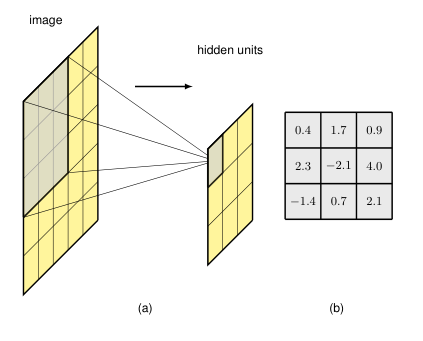
\includegraphics[width=0.2\textwidth]{ch10-2-1/figure-10-1.png}
        \caption{(a) 感受野 $3 \times 3$；(b) 权重可视化为核。}
    \end{figure}
\end{frame}

\begin{frame}
    \frametitle{2.1 滤波器作为模板匹配器}
    \begin{itemize}
        \item 假设 $\mathbf{w}$ 和 $w_0$ 固定，问什么输入 $\mathbf{x}$ 给出最大响应？
        \item 约束 $\|\mathbf{x}\|^2$ 固定，最大化 $\mathbf{w}^T\mathbf{x}$ 的解：
        \begin{equation}
            \mathbf{x} = \alpha\mathbf{w}
        \end{equation}
        \item \textbf{含义}：最大响应出现在图像块\alert{看起来像滤波器图像}时（允许整体缩放）。
        \item ReLU 仅在 $\mathbf{w}^T\mathbf{x} > -w_0$ 时产生非零输出。
        \item 单元充当\alert{特征检测器}：找到足够好的匹配时发出信号。
    \end{itemize}
\end{frame}

% ============================================================
% 第三部分：平移等变性
% ============================================================
\section{平移等变性}

\begin{frame}
    \frametitle{3. 平移等变性 (10.2.2)}
    \begin{itemize}
        \item 若某位置的小块表示眼睛，则其他位置的相同像素值也表示眼睛。
        \item 网络需\alert{泛化到所有位置}，无需每个位置都有训练样本。
        \item \textbf{方法}：在图像多个位置\alert{复制相同的权重值}。
    \end{itemize}
    \begin{figure}
        \centering
        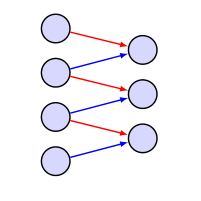
\includegraphics[width=0.15\textwidth]{ch10-2-2/figure-10-2.png}
        \caption{一维卷积：6 个连接，仅 2 个独立可学习参数。}
    \end{figure}
    \begin{itemize}
        \item 隐藏层单元构成\alert{特征图}，所有单元\alert{共享权重}。
        \item 图像某块产生特定响应 $\Rightarrow$ 平移后相同像素值在特征图相应平移位置产生相同响应。
        \item 这就是\alert{等变性}。
    \end{itemize}
\end{frame}

\begin{frame}
    \frametitle{3.1 卷积的两大核心特性}
    \begin{block}{稀疏连接 (Sparse Connections)}
        大多数连接不存在，减少权重数量。
    \end{block}
    \begin{block}{参数共享 (Parameter Sharing)}
        所有权重值由所有隐藏单元共享，大幅减少独立参数。
    \end{block}
    \begin{itemize}
        \item 这种变换称为\alert{卷积}。
    \end{itemize}
\end{frame}

\begin{frame}
    \frametitle{3.2 二维卷积的数学定义}
    图像 $\mathbf{I}$（像素 $I(j,k)$），滤波器 $\mathbf{K}$（像素 $K(l,m)$），特征图 $\mathbf{C}$：
    \begin{equation}
        C(j, k) = \sum_l \sum_m I(j + l, k + m)K(l, m)
        \tag{10.2}
    \end{equation}
    \begin{itemize}
        \item 可表示为 $\mathbf{C} = \mathbf{I} * \mathbf{K}$。
        \item 严格来说是\alert{互相关}，但机器学习文献惯例称为卷积。
        \item 图 10.3：$3 \times 3$ 图像 + $2 \times 2$ 滤波器 $\to$ $2 \times 2$ 特征图。
    \end{itemize}
    \begin{block}{批归一化的特殊要求}
        卷积网络中使用批归一化时，\alert{特征图内每个空间位置}必须使用相同的均值和方差。\\
        确保特征图统计特性\alert{与位置无关}。
    \end{block}
\end{frame}

\begin{frame}
    \frametitle{3.3 手工设计的边缘检测滤波器}
    垂直边缘检测（$3 \times 3$ 滤波器）：
    \begin{equation}
        \begin{bmatrix} -1 & 0 & 1 \\ -1 & 0 & 1 \\ -1 & 0 & 1 \end{bmatrix}
        \tag{10.3}
    \end{equation}
    水平边缘检测（转置）：
    \begin{equation}
        \begin{bmatrix} -1 & -1 & -1 \\ 0 & 0 & 0 \\ 1 & 1 & 1 \end{bmatrix}
        \tag{10.4}
    \end{equation}
    \begin{itemize}
        \item 直观：水平扫过图像时强度显著局部变化 $\Rightarrow$ 垂直边缘。
        \item 正权重对应右/下像素，负权重对应左/上像素 $\Rightarrow$ 方向性导数。
    \end{itemize}
\end{frame}

\begin{frame}
    \frametitle{3.4 边缘检测结果的正负响应}
    \begin{figure}
        \centering
        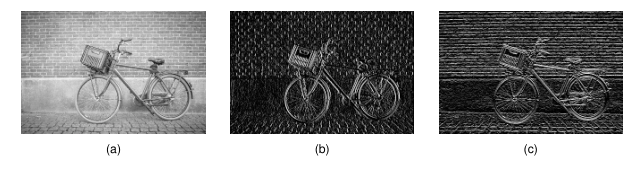
\includegraphics[width=0.5\textwidth]{ch10-2-2/figure-10-4.png}
        \caption{(a) 原图；(b) 垂直边缘检测；(c) 水平边缘检测。}
    \end{figure}
    \begin{itemize}
        \item 垂直边缘对应\alert{强度增加} $\Rightarrow$ 特征图对应点\alert{为正}（亮色）。
        \item 垂直边缘对应\alert{强度减小} $\Rightarrow$ 特征图对应点\alert{为负}（暗色）。
        \item 水平边缘类似。
    \end{itemize}
\end{frame}

\begin{frame}
    \frametitle{3.5 卷积结构相对全连接的三大优势}
    \begin{enumerate}
        \item \alert{稀疏连接}：即使大图像也只需很少权重。
        \item \alert{权重共享}：大幅减少独立参数 $\Rightarrow$ 降低训练集大小需求。
        \item \alert{输入尺寸灵活}：相同网络可应用于不同尺寸图像，无需重新训练。
        \begin{itemize}
            \item 改变输入尺寸只改变特征图大小，\alert{不改变权重数量}。
        \end{itemize}
    \end{enumerate}
    \begin{block}{GPU 并行}
        卷积操作在大量位置上重复，特别适合 GPU 大规模并行，实现高计算吞吐。
    \end{block}
\end{frame}

% ============================================================
% 第四部分：填充与跨步卷积
% ============================================================
\section{填充与跨步卷积}

\begin{frame}
    \frametitle{4. 填充 (Padding, 10.2.3)}
    \begin{itemize}
        \item 卷积映射比原图小：$J \times K$ 图像 + $M \times M$ 核 $\to$ $(J-M+1) \times (K-M+1)$。
        \item 若希望输出与输入\alert{尺寸相同}：填充 $P$ 个像素。
        \begin{itemize}
            \item 输出：$(J+2P-M+1) \times (K+2P-M+1)$
        \end{itemize}
        \item \alert{有效卷积}：$P = 0$，输出缩小。
        \item \alert{相同卷积}：$P = (M-1)/2$，输出与输入同尺寸。
        \item 滤波器通常用\alert{奇数} $M$：对称填充 + 明确定义的中心像素。
        \item 填充值通常设\alert{零}（配合图像零均值化）。
        \item 填充也可应用于特征图，供后续卷积层处理。
    \end{itemize}
\end{frame}

\begin{frame}
    \frametitle{4.1 跨步卷积 (Strided Convolutions, 10.2.4)}
    \begin{itemize}
        \item 大图像 + 小核 $\Rightarrow$ 特征图与原图相近。
        \item 有时希望特征图\alert{显著更小}，为架构设计提供灵活性。
        \item \alert{跨步卷积}：滤波器以步长 $S$ 移动（而非 1 像素）。
        \item 水平和垂直同一步长时，特征图元素数量：
        \begin{equation}
            \left\lfloor \frac{J + 2P - M}{S} - 1 \right\rfloor \times \left\lfloor \frac{K + 2P - M}{S} - 1 \right\rfloor
            \tag{10.5}
        \end{equation}
        \item 大图像 + 小滤波器：特征图约为原图的 $1/S$。
        \item 核心功能：\alert{下采样}，减少空间尺寸。
    \end{itemize}
\end{frame}

% ============================================================
% 第五部分：多维卷积
% ============================================================
\section{多维卷积}

\begin{frame}
    \frametitle{5. 多通道输入的卷积 (10.2.5)}
    \begin{itemize}
        \item 彩色图像：3 通道（红、绿、蓝）。
        \item 扩展滤波器维度以覆盖多通道。
        \item 图像：$J \times K \times C$ 的\alert{张量}。
        \item 滤波器：$M \times M \times C$ 的张量，每个输入通道一个 $M \times M$ 滤波器。
        \item 无填充、步长 1：特征图 $(J-M+1) \times (K-M+1)$。
    \end{itemize}
    \begin{figure}
        \centering
        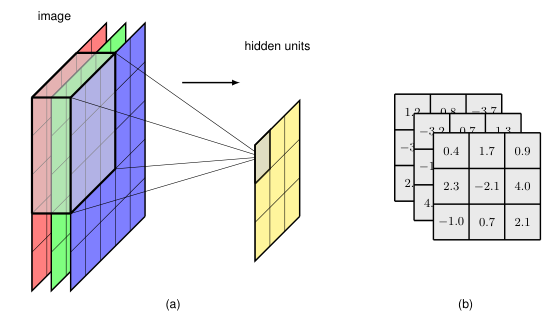
\includegraphics[width=0.25\textwidth]{ch10-2-5/figure-10-6.png}
        \caption{(a) 多维滤波器；(b) $3 \times 3 \times 3$ 张量，27 个权重。}
    \end{figure}
\end{frame}

\begin{frame}
    \frametitle{5.1 多输出通道}
    \begin{itemize}
        \item 单滤波器 $\approx$ 全连接网络中的单个隐藏节点，只能检测\alert{一种特征}。
        \item \textbf{扩展}：包含\alert{多个滤波器}，每个有独立参数和独立特征图。
        \item 这些独立特征图也称为\alert{通道}。
        \item 滤波器张量：$M \times M \times C \times C_{\text{OUT}}$
        \begin{itemize}
            \item $C$：输入通道数
            \item $C_{\text{OUT}}$：输出通道数
        \end{itemize}
        \item 总参数数量：$(M^2C + 1)C_{\text{OUT}}$
        \item \textbf{关键}：参数量与\alert{输入图像空间尺寸无关}。
    \end{itemize}
\end{frame}

\begin{frame}
    \frametitle{5.2 $1 \times 1$ 卷积}
    \begin{itemize}
        \item 滤波器尺寸为\alert{单个像素}的卷积层。
        \item 滤波器有 $C$ 个权重（每个输入通道一个）+ 一个偏置。
        \item \textbf{应用}：改变通道数量（通常减少），\alert{不改变特征图空间尺寸}。
        \item 与跨步卷积或池化\alert{互补}：
        \begin{itemize}
            \item $1 \times 1$ 卷积：减少\alert{通道数}
            \item 跨步卷积/池化：减少\alert{空间维度}
        \end{itemize}
        \item 本质：跨通道的全连接层（对每个位置独立应用）。
    \end{itemize}
\end{frame}

% ============================================================
% 第六部分：池化
% ============================================================
\section{池化}

\begin{frame}
    \frametitle{6. 池化 (Pooling, 10.2.6)}
    \begin{itemize}
        \item 卷积层编码\alert{平移等变性}：特征平移 $\Rightarrow$ 特征图相应平移。
        \item 适用于\alert{定位}任务（如找物体位置）。
        \item 但\alert{分类}任务希望输出对平移\alert{不变}。
        \item 需要层级结构，但简单特征的\alert{微小相对位置变化}不应影响分类。
        \item \textbf{解决方案}：对卷积层输出应用\alert{池化}。
    \end{itemize}
    \begin{block}{等变性 vs 不变性}
        \begin{itemize}
            \item 等变性：输出随输入平移而\alert{同步平移}
            \item 不变性：输出对平移\alert{不敏感}
        \end{itemize}
    \end{block}
\end{frame}

\begin{frame}
    \frametitle{6.1 最大池化}
    \begin{itemize}
        \item 池化结构与卷积类似：网格排列，每个单元有感受野。
        \item 需选择滤波器尺寸和步长。
        \item \textbf{关键区别}：池化输出是输入的\alert{简单固定函数}，\alert{无可学习参数}。
        \item \alert{最大池化}：每个单元输出输入值的\alert{最大值}。
    \end{itemize}
    \begin{figure}
        \centering
        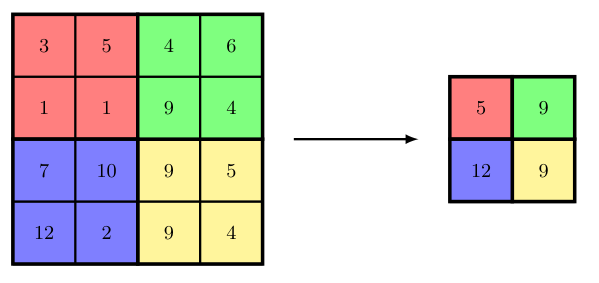
\includegraphics[width=0.45\textwidth]{ch10-2-6/figure-10-8.png}
        \caption{$2 \times 2$ 块用 max 运算符合并，生成更小特征图。}
    \end{figure}
\end{frame}

\begin{frame}
    \frametitle{6.2 池化的功能与类型}
    \begin{itemize}
        \item \textbf{双重功能}：
        \begin{enumerate}
            \item 引入局部\alert{平移不变性}
            \item 通过\alert{下采样}降低表示维度
        \end{enumerate}
        \item 卷积层步长 > 1 也有下采样效果（但可学习）。
        \item 特征图激活值 = 特征检测强度。
        \begin{itemize}
            \item 最大池化：保留“特征是否存在”及强度，\alert{丢弃部分位置信息}。
        \end{itemize}
        \item 其他池化函数：\alert{平均池化}（计算感受野平均值）。
        \item 所有池化都引入一定程度的\alert{局部平移不变性}。
    \end{itemize}
\end{frame}

\begin{frame}
    \frametitle{6.3 通道独立池化与跨通道池化}
    \begin{block}{通道独立池化}
        池化通常\alert{独立应用于每个通道}。
        \begin{itemize}
            \item 例：8 通道 $64 \times 64$ 特征图，$2 \times 2$ 最大池化步长 2
            \item 输出：$32 \times 32 \times 8$
            \item 池化\alert{不改变通道数}，只改变空间维度。
        \end{itemize}
    \end{block}
    \begin{block}{跨通道池化}
        对特征图的\alert{多个通道}进行池化。
        \begin{itemize}
            \item 使网络能\alert{学习}除平移外的其他不变性。
            \item 例：多个通道检测同一特征的不同朝向，跨通道最大池化 $\approx$ \alert{旋转不变性}。
        \end{itemize}
    \end{block}
\end{frame}

\begin{frame}
    \frametitle{6.4 池化适应变尺寸图像}
    \begin{itemize}
        \item 卷积网络最终输出（及部分中间层）必须有\alert{固定尺寸}。
        \item \textbf{问题}：如何用同一网络处理不同尺寸图像？
        \item \textbf{方法}：根据图像尺寸\alert{调整池化步长}。
        \begin{itemize}
            \item 使池化输出的数量保持\alert{恒定}。
            \item 从而适配可变尺寸输入。
        \end{itemize}
        \item 注意：步长变化改变感受野覆盖密度，可能影响特征提取的尺度一致性。
    \end{itemize}
\end{frame}

% ============================================================
% 第七部分：多层卷积与经典架构
% ============================================================
\section{多层卷积与经典架构}

\begin{frame}
    \frametitle{7. 多层卷积 (10.2.7)}
    \begin{itemize}
        \item 单层卷积 $\approx$ 全连接网络的单层。
        \item 堆叠多层 $\Rightarrow$ 发现和表达\alert{层次化结构}。
        \item 每个卷积层：
        \begin{itemize}
            \item 滤波器张量 $M \times M \times C_{\text{IN}} \times C_{\text{OUT}}$
            \item 参数量 $(M^2C_{\text{IN}} + 1)C_{\text{OUT}}$
        \end{itemize}
        \item 每个卷积层后可选跟\alert{池化层}。
        \item 某层 $C_{\text{OUT}}$ 个输出通道 $\to$ 下一层的输入通道。
        \item 术语注意：通道数有时称“深度”，但本书保留“深度”表示\alert{层数}。
    \end{itemize}
\end{frame}

\begin{frame}
    \frametitle{7.1 感受野随深度增长}
    \begin{itemize}
        \item 关键属性：\alert{局部性}——每个单元只从上一层小区域取信息。
        \item 深层网络中，后层单元的有效感受野\alert{远大于}早期层。
    \end{itemize}
    \begin{figure}
        \centering
        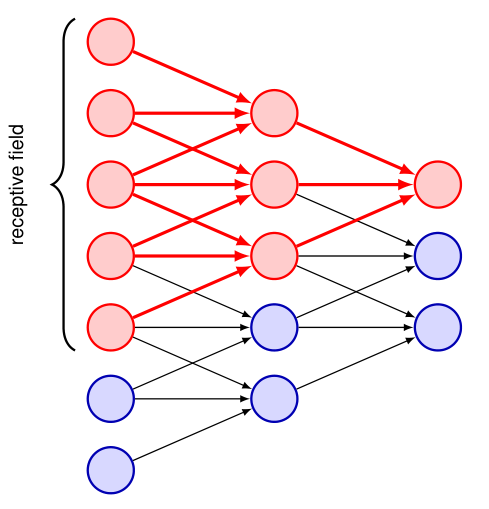
\includegraphics[width=0.15\textwidth]{ch10-2-7/figure-10-9.png}
        \caption{有效感受野随深度增长。}
    \end{figure}
    \begin{itemize}
        \item 不增加参数，通过\alert{层级组合}自然扩大视野。
        \item 这是深度卷积网络捕捉全局上下文的基础。
    \end{itemize}
\end{frame}

\begin{frame}
    \frametitle{7.2 全连接层作为输出阶段}
    \begin{itemize}
        \item 分类等任务需对\alert{整张图像}做预测。
        \item 通常引入 1--2 个\alert{全连接层}作为网络最后阶段。
        \item 每层单元与上一层所有单元相连。
        \item 参数量可管理：因池化使最终卷积层维度远低于输入层。
        \item \textbf{注意}：最终全连接层可能包含网络中\alert{大部分独立参数}。
        \begin{itemize}
            \item 即使卷积层（共享）连接数更多。
        \end{itemize}
    \end{itemize}
\end{frame}

\begin{frame}
    \frametitle{7.3 完整 CNN 架构设计}
    \begin{itemize}
        \item 完整 CNN：
        \begin{itemize}
            \item 多个卷积层 + 池化操作
            \item 最后阶段常有传统全连接层
        \end{itemize}
        \item 设计选择（超参数）：
        \begin{itemize}
            \item 层数、每层通道数
            \item 滤波器尺寸、步长宽度
            \item 等多个超参数
        \end{itemize}
        \item \textbf{困难}：训练成本高，难以用留出数据系统比较。
        \item 已探索各种架构，依赖经验法则和迁移已有成功架构。
    \end{itemize}
\end{frame}

\begin{frame}
    \frametitle{7.4 早期成功与 ImageNet (10.2.8)}
    \begin{itemize}
        \item CNN 是首批成功部署的\alert{深度神经网络}。
        \item \alert{LeNet}：低分辨率手写数字灰度图像分类。
        \item \alert{ImageNet} 推动发展：
        \begin{itemize}
            \item 约 1400 万张自然图像
            \item 近 22,000 个类别
            \item 远超此前数据集规模
        \end{itemize}
        \item 强调\alert{大规模数据} + \alert{适当归纳偏置}的模型的重要性。
    \end{itemize}
\end{frame}

\begin{frame}
    \frametitle{7.5 ImageNet 挑战赛与 AlexNet}
    \begin{itemize}
        \item 子集：1000 个不重叠类别。
        \item 随机猜测错误率：99.9%。
        \item 数据：128 万训练 + 5 万验证 + 10 万测试。
        \item 评价：\alert{top-1} 和 \alert{top-5} 错误率。
        \item 早期结果：top-5 错误率约 25.5%。
    \end{itemize}
    \begin{block}{AlexNet (2012) 突破}
        赢得 2012 年比赛，top-5 错误率降至 \alert{15.3\%}。
        \begin{itemize}
            \item \alert{ReLU} 激活函数
            \item \alert{GPU} 训练
            \item \alert{Dropout} 正则化
        \end{itemize}
        后续年份错误率降至约 3\%，优于人类约 5\% 的水平。
    \end{block}
\end{frame}

\begin{frame}
    \frametitle{7.6 VGG-16 架构详解}
    \begin{itemize}
        \item VGG = Visual Geometry Group，16 = 可学习层数。
        \item 输入：$224 \times 224 \times 3$。
        \item 设计原则：\alert{统一架构}，最小化超参数选择。
        \item 所有卷积层：$3 \times 3$ 滤波器，步长 1，same padding，ReLU。
        \item 所有最大池化：步长 2，$2 \times 2$ 滤波器（下采样 4 倍）。
        \item 通道数变化：64 $\to$ 128 $\to$ 256 $\to$ 512
        \begin{itemize}
            \item 下采样时\alert{通道数加倍}，平衡表示容量。
        \end{itemize}
        \item 最后 3 层\alert{全连接}：4096, 4096, 1000。
        \item 总参数：约 \alert{1.38 亿}。
        \begin{itemize}
            \item 近 1.03 亿在\alert{第一个全连接层}。
            \item 大部分连接在第一个卷积层。
        \end{itemize}
    \end{itemize}
\end{frame}

\begin{frame}
    \frametitle{7.7 小卷积核堆叠的优势}
    \begin{itemize}
        \item 早期 CNN：较大感受野（如 AlexNet $11 \times 11$，步长 4）。
        \item 大感受野也可通过\alert{多层小感受野}隐式实现。
        \item \textbf{优势}：
        \begin{itemize}
            \item 参数显著更少
            \item 对较大滤波器施加归纳偏置（必须由卷积子滤波器组合）
        \end{itemize}
        \item 尽管架构复杂，只需编码\alert{网络函数本身}：
        \begin{itemize}
            \item 导数用\alert{自动微分}计算
            \item 代价函数用\alert{随机梯度下降}优化
        \end{itemize}
    \end{itemize}
\end{frame}

% ============================================================
% 第八部分：总结
% ============================================================
\section{总结}

\begin{frame}
    \frametitle{8. 本节总结}
    \begin{itemize}
        \item \alert{动机}：全连接网络参数爆炸，需融入图像结构归纳偏置。
        \item \alert{四大概念}：层级性、局部性、等变性、不变性。
        \item \alert{感受野与滤波器}：局部输入区域，权重可视化为核。
        \item \alert{滤波器 = 模板匹配器}：最大响应于与核形状一致的输入。
        \item \alert{平移等变性}：权重复制实现位置泛化。
        \item \alert{卷积两大特性}：稀疏连接、参数共享。
        \item \alert{填充}：有效卷积 vs 相同卷积。
        \item \alert{跨步卷积}：下采样，减少空间尺寸。
        \item \alert{多维卷积}：多输入通道 + 多输出通道。
        \item \alert{$1 \times 1$ 卷积}：通道维度变换。
        \item \alert{池化}：平移不变性 + 降维，无可学习参数。
        \item \alert{多层卷积}：感受野随深度增长，全连接层作为输出阶段。
        \item \alert{经典架构}：LeNet, AlexNet, VGG-16。
    \end{itemize}
\end{frame}

% ============================================================
% 第九部分：参考文献
% ============================================================
\section{参考文献}

\begin{frame}
    \frametitle{9. 参考文献}
    \begin{itemize}
        \item 教材：Bishop, C. M. \& Bishop, H. (2023). Deep Learning Foundations and Concepts. Springer Nature Switzerland AG.
        \item LeCun, Y. et al. (1998). Gradient-based learning applied to document recognition.
        \item Krizhevsky, A., Sutskever, I., \& Hinton, G. E. (2012). ImageNet classification with deep convolutional neural networks.
        \item Simonyan, K. \& Zisserman, A. (2014). Very deep convolutional networks for large-scale image recognition.
        \item Dumoulin, V. \& Visin, F. (2016). A guide to convolution arithmetic for deep learning.
        \item Lin, M., Chen, Q., \& Yan, S. (2013). Network in network.
    \end{itemize}
\end{frame}

\end{document}